
\section{Simulation}\label{sec:simulation}


\subsection{1D mapping}

 Simulations were conducted in Mathematica, code at github \cite{Arun2017GitHubUniformMapping}. 
 Fig.~\ref{fig:Prob1DcoverageGaps} shows the distributions for the minimum and maximum initial particle locations $\underline{p}$ and $\overline{p}$, the maximum gap $\overline{g}$, and the spread between the minimum and maximum $\overline{p}-\underline{p}$ for 1,000,000 Monte Carlo trials.
 The expected gap between the first particle and the boundary $\underline{p}$ is 90.94.
 The expected gap between the last particle and the boundary $\overline{p}$ is 90.98.
  The expected maximum gap is $\overline{g}$ is 273.9.
  
  
  \subsection{2D mapping}  
  The mapping simulation was repeated 100 times for a given number of particles in a map with 5000 free spaces. 
  In each run the particles were placed randomly throughout the workspace. 
  For smaller ratios of particles/workspace the standard deviation of the completion time is large. 
  As the number of particles increases from 100 to 5000 by increments of 100, the deviation decreases. 
  The function of moves vs.\ number of particles is an exponentially decreasing curve. 
  %The legend will be changed in pdf image to have italics. 
  A comparison between the simulation results of the three algorithms is shown in  Fig.~\ref{fig:Alg_linlogplot}. 
  The log plot shows that all three algorithms have a almost logarithmic relationship between the number of free space $m$ and number of particles $k$.  
  The maximum number of moves required using the Closest Frontier algorithm was for $k$=100 with an average moves $\approx$1816 and standard deviation of 160 moves.
This reduces to  four moves with 0 standard deviation when $n$= 5000 (the total number of free spaces).
  

  	The comparison plot between the mapping of the three maps� \emph{complex}, \emph{empty rectangle} and \emph{linear} shows that the complex map requires the most moves. 
	In the Fig.~\ref{fig:MappingAlg3maps} there is an observable difference in moves between the linear and rectangular workspaces. 
	One reason is because the number of useful moves is reduced in the linear case, where only left and right are useful moves. 
	Up and down eliminate boundaries, but never discover free cells. 
	%Nevertheless, it is important to identify the boundary. 
	Whereas in the \emph{empty rectangle} case most of the moves are moves which add to the number of mapped spaces. 
	Only when the number of particles is around 2/3 of the number of free spaces is there an overlap between the moves taken to map the rectangular space and the linear space. 
	
%	We should look at bounding the complexity. 
  	
%  	\todo{insert observation values for the number of moves in three maps. Insert comparison between 3 algorithms random, elect and nearest node. Insert comparison between flood fill, uniform distribution and regional distribution.} 

\begin{figure}
\begin{center}
	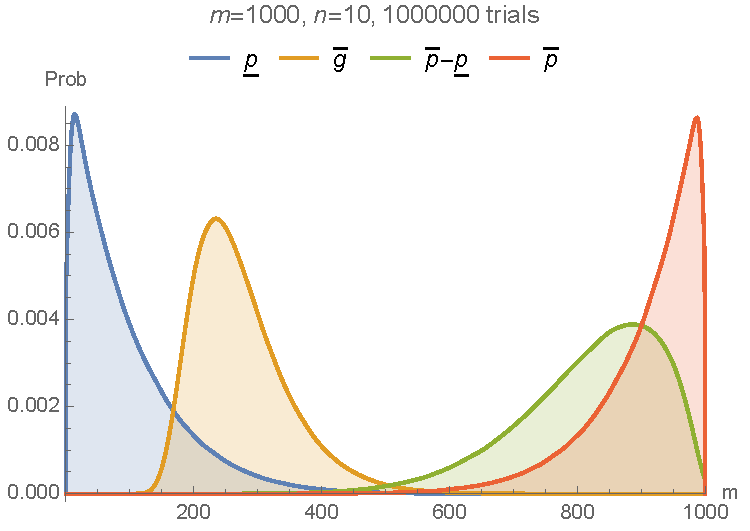
\includegraphics[width=1.0\columnwidth]{Prob1DcoverageGaps}
\end{center}
\caption{\label{fig:Prob1DcoverageGaps}
With a connected freespace $m$ = 1000 and $n=10$ particles, the distributions for the gap before the first $\overline{p}$ and after the last $\underline{p}$  gaps are symmetric. The maximum gap $\overline{g} \approx 250$.}
\end{figure}


\begin{figure}
\begin{center}
	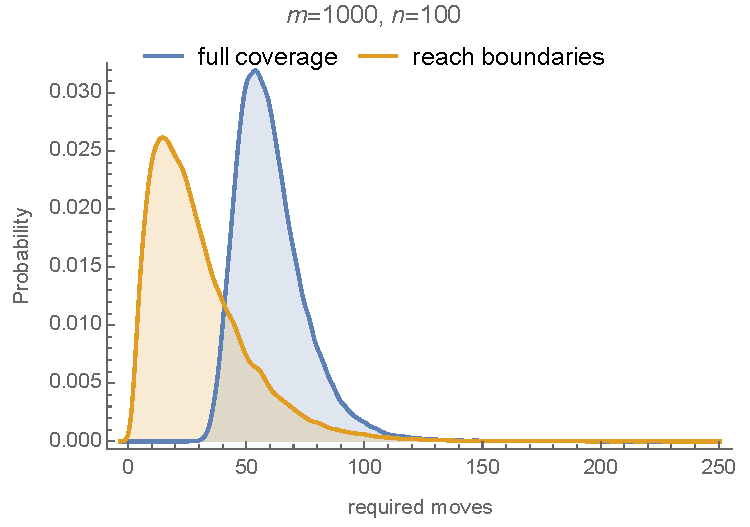
\includegraphics[width=1.0\columnwidth]{SimReachBoundaryCoverage}
\end{center}
\caption{\label{fig:SimReachBoundaryCoverage}
Full coverage requires 60.7 moves on average, while reaching the boundaries requires only 29.8.}
\end{figure}


%\begin{figure}
%\begin{center}
%	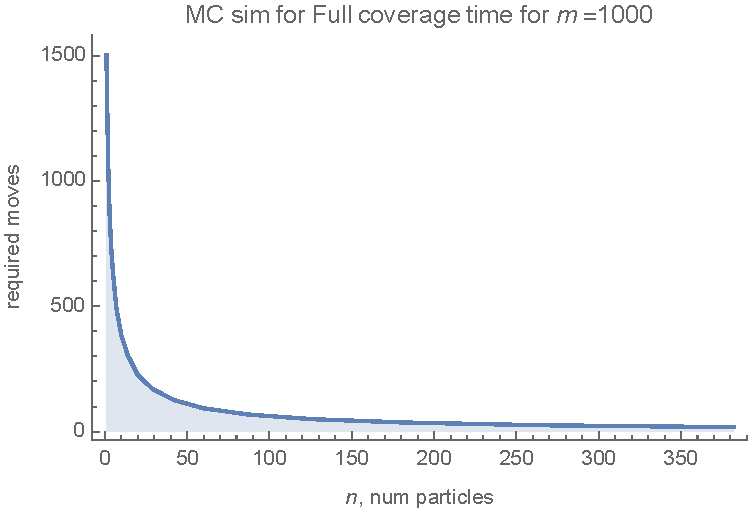
\includegraphics[width=1.0\columnwidth]{Sim1DCoverageFuncOfn}
%\end{center}
%\caption{\label{fig:Sim1DCoverageFuncOfn}
%Number of required moves for full coverage in 1D  as a function of $n$ for $m=1000$.}
%\end{figure}

%\begin{figure}
%\begin{center}
%	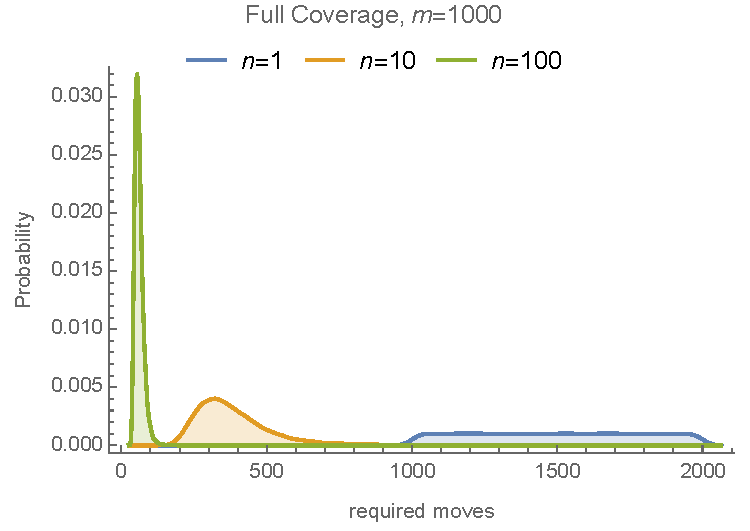
\includegraphics[width=1.0\columnwidth]{SimFullCoverageVaryn}
%\end{center}
%\caption{\label{fig:SimFullCoverageVaryn}
%Probability distributions for required number of moves for different numbers of particles $n$.}
%\end{figure}

\begin{figure}
\begin{center}
	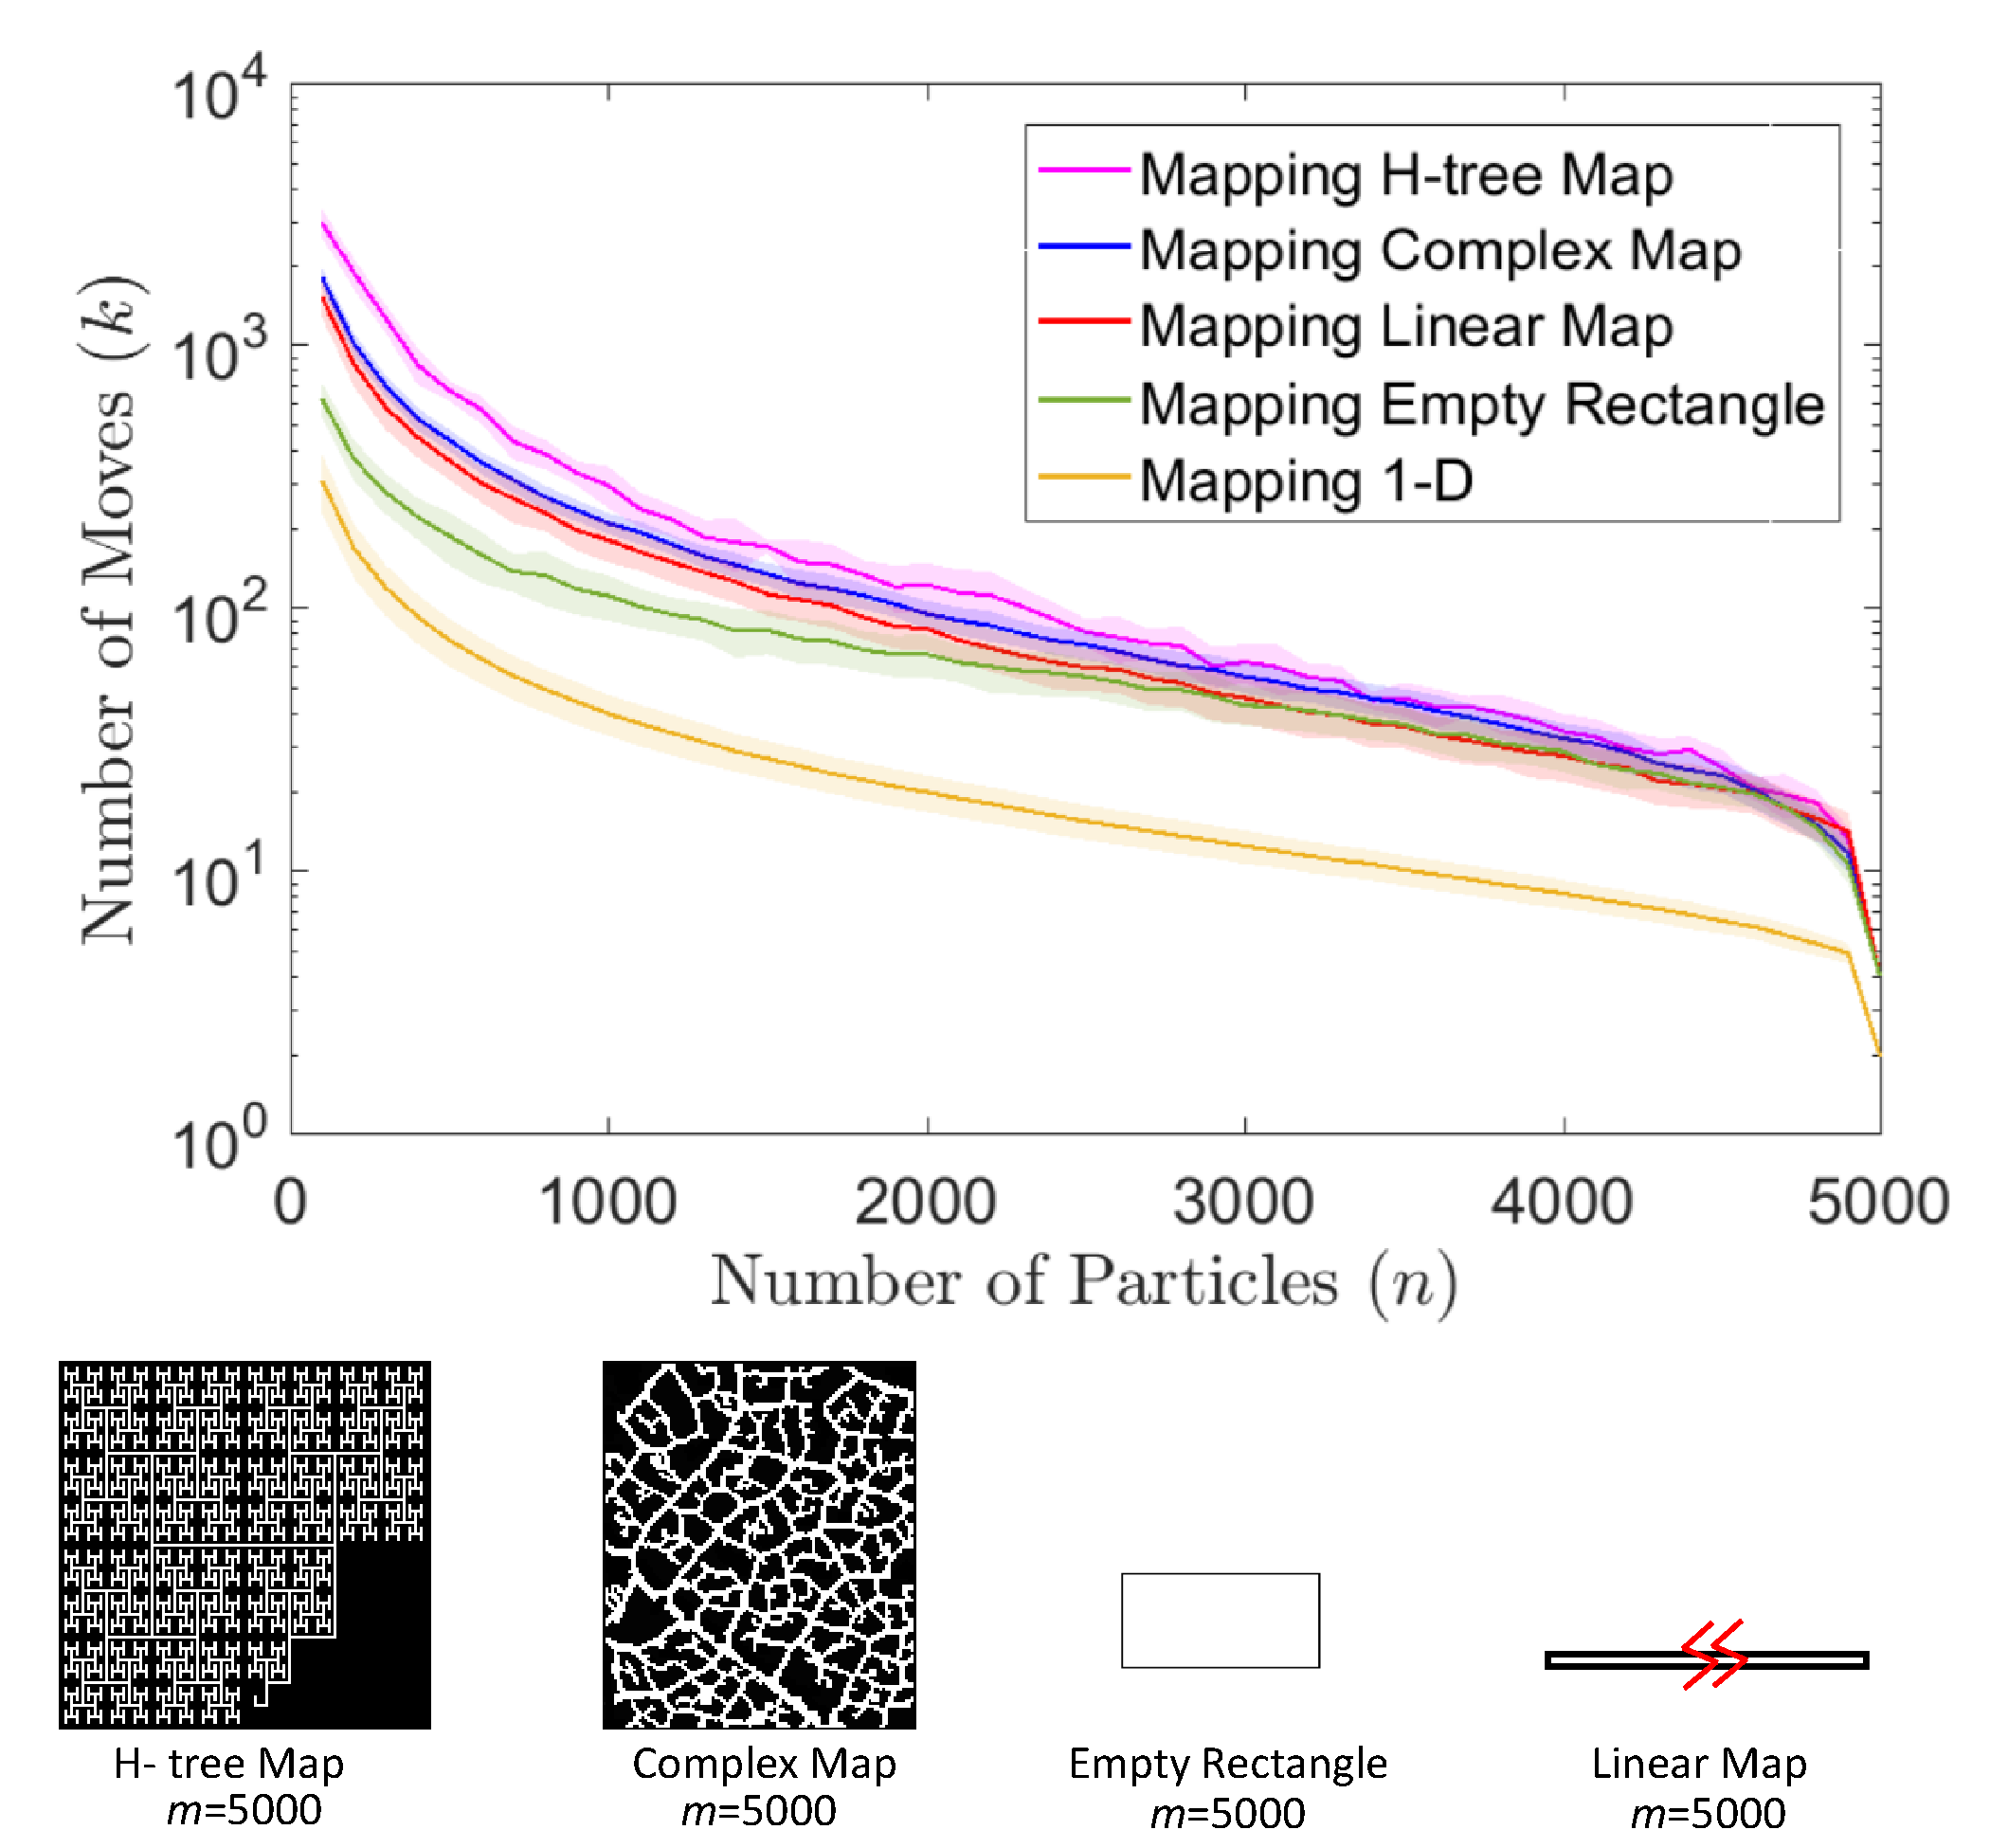
\includegraphics[width=1.0\columnwidth]{MappingAlg3maps}
\end{center}
\caption{\label{fig:MappingAlg3maps}
Comparison of mapping 2D maps of three types using the Closest Frontier algorithm and the 1-D mapping of the linear map. The complex map, empty rectangle map, and linear map (similar to a 1D map, but with obstacles to detect on top and bottom) have 5000 free spaces.
}
\end{figure}
\begin{figure}
\begin{center}
	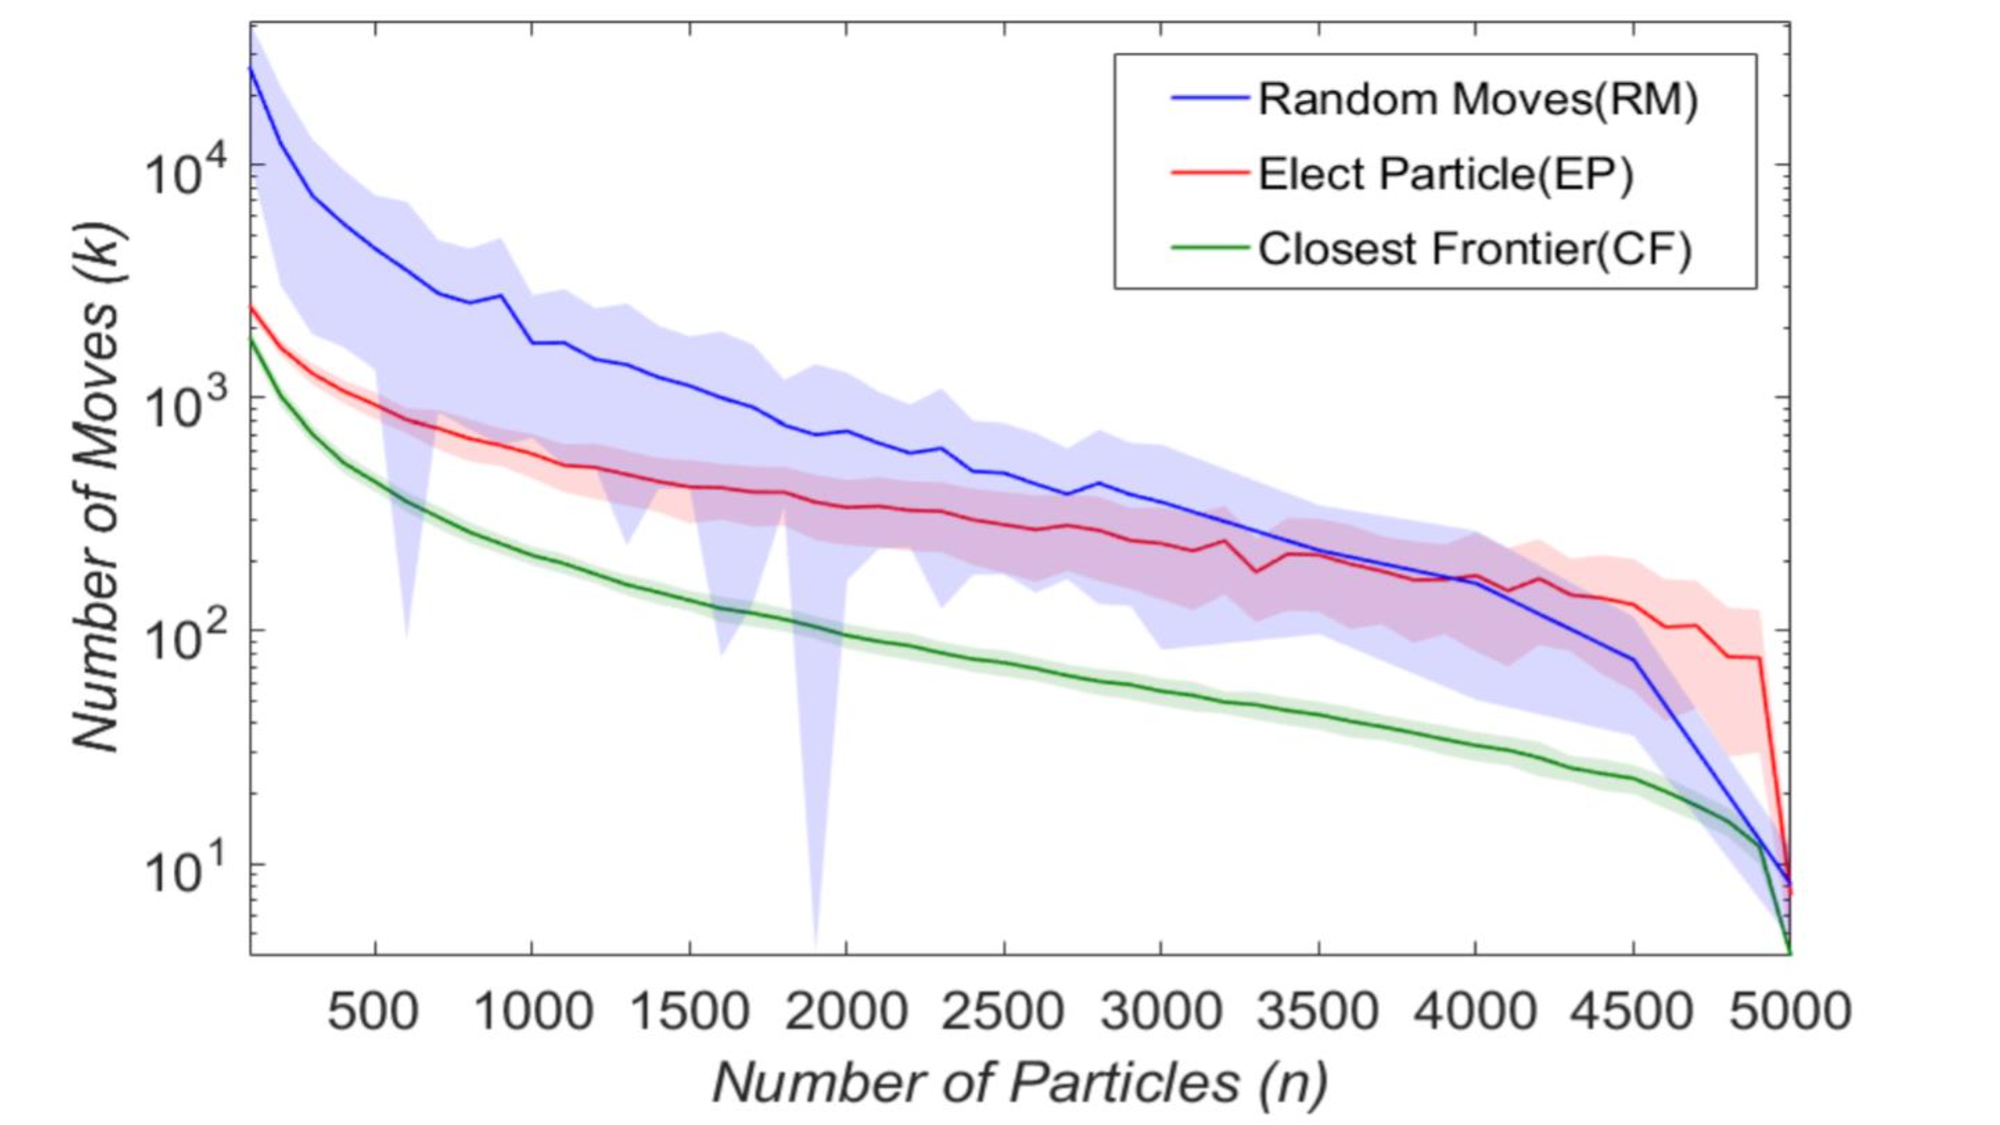
\includegraphics[width=1.0\columnwidth]{Alg_linlogplot}
\end{center}
\caption{\label{fig:Alg_linlogplot}
Comparison of three Algorithms - Random Moves (Blue), Elect Particle (Red) and Closest Frontier (Green) for mapping the 2D Complex Map of 5000 free spaces.}
\end{figure}


\begin{figure}
\begin{center}
	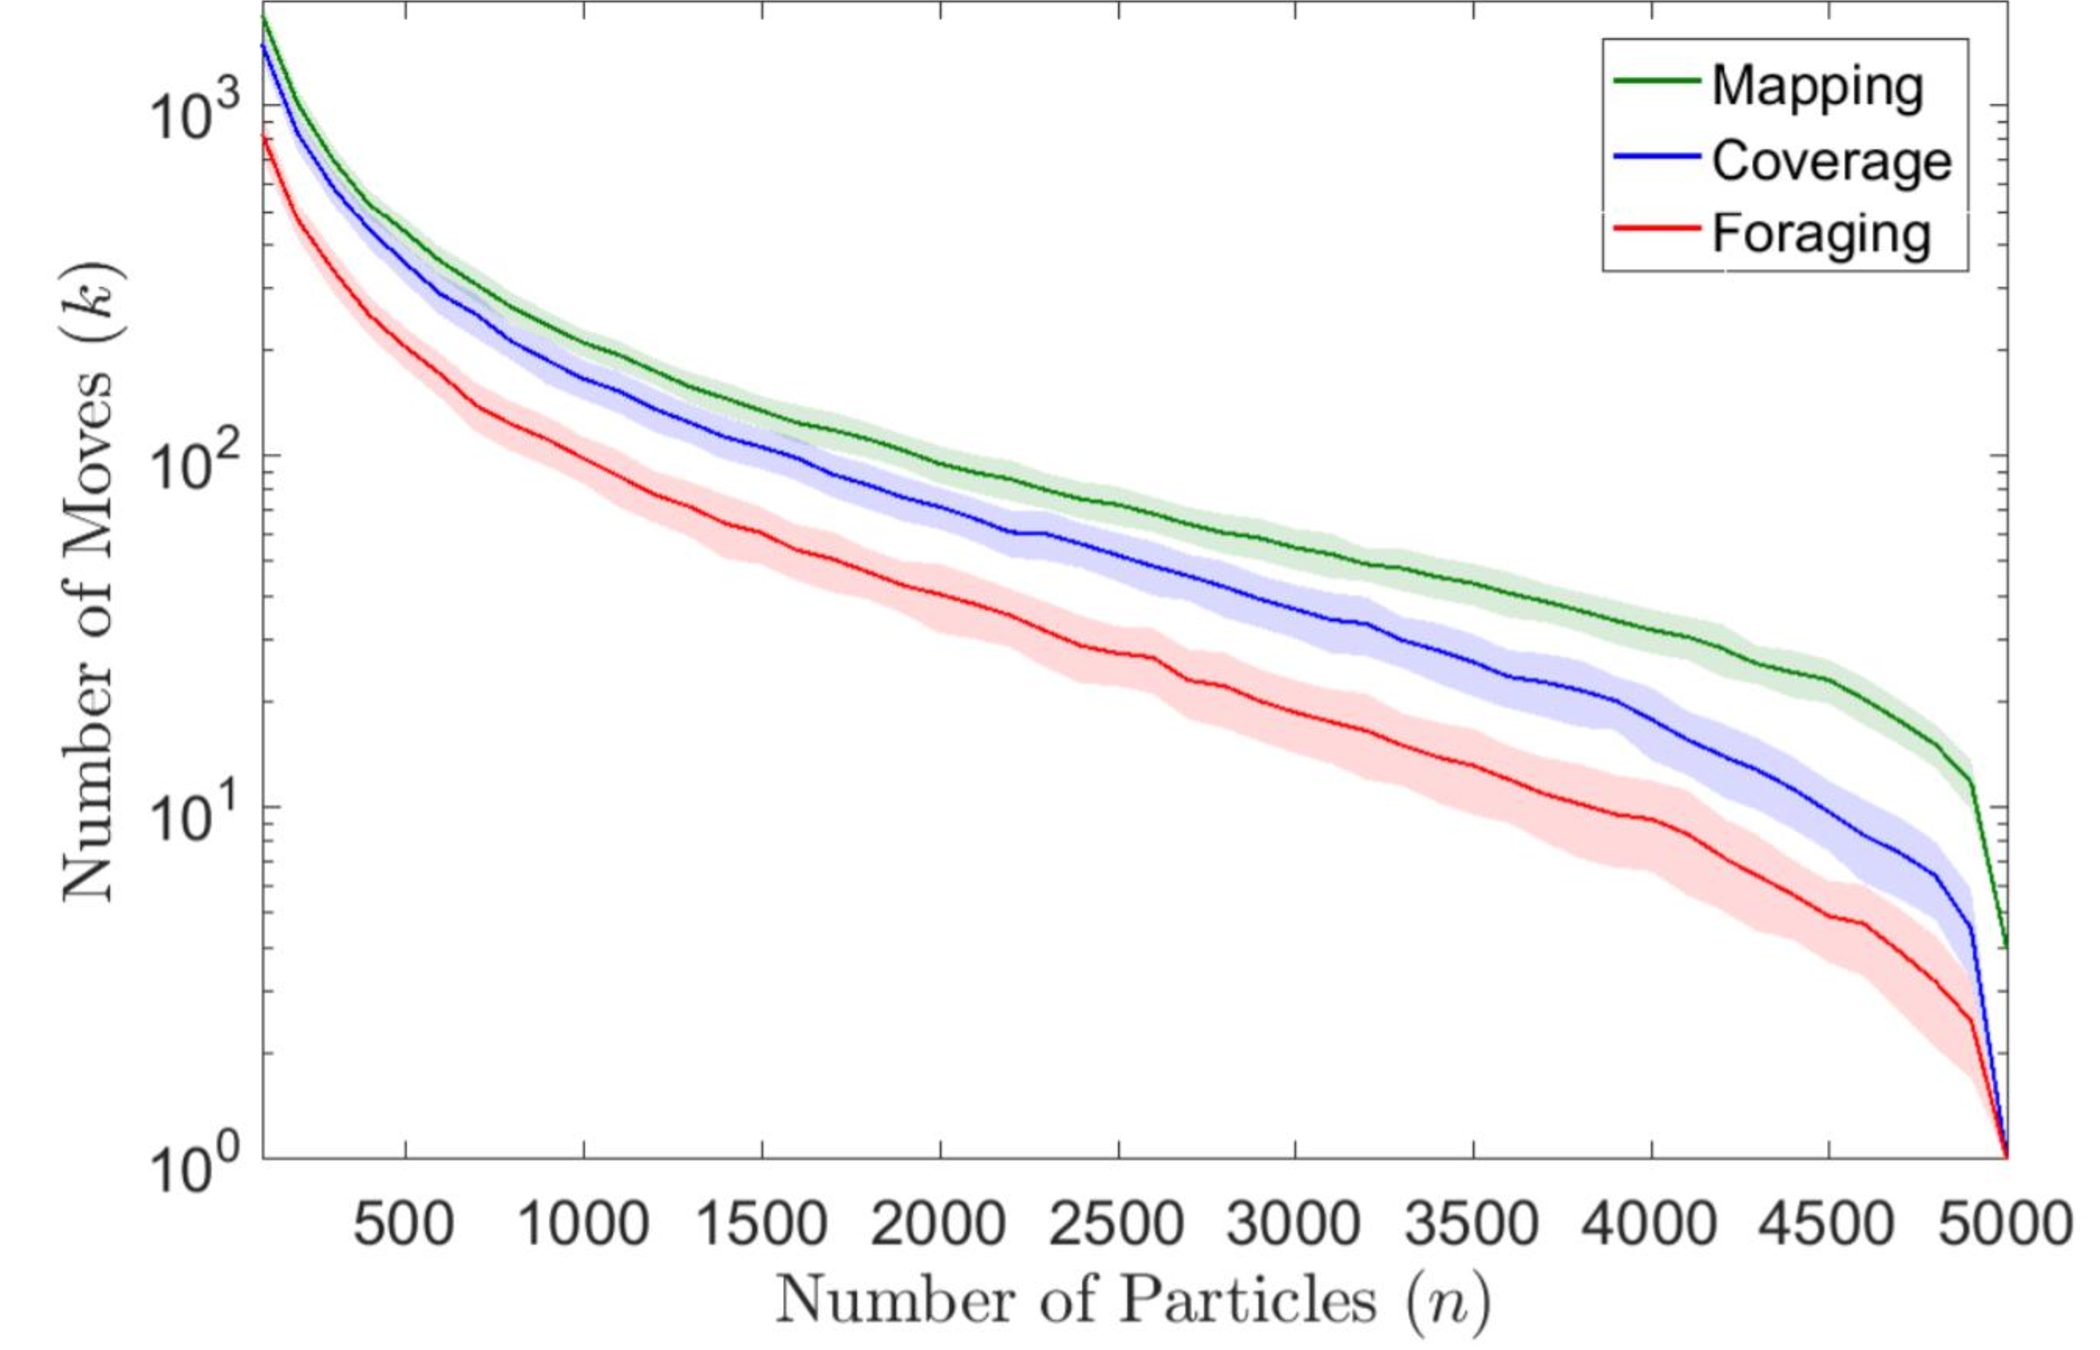
\includegraphics[width=1.0\columnwidth]{CoverageMappingForaging.pdf}
\end{center}
\caption{\label{fig:CoverageMappingForaging}
Comparison of three related problems: coverage, mapping, and foraging on the complex 2D map.}
\end{figure}

\begin{figure}
\begin{center}
	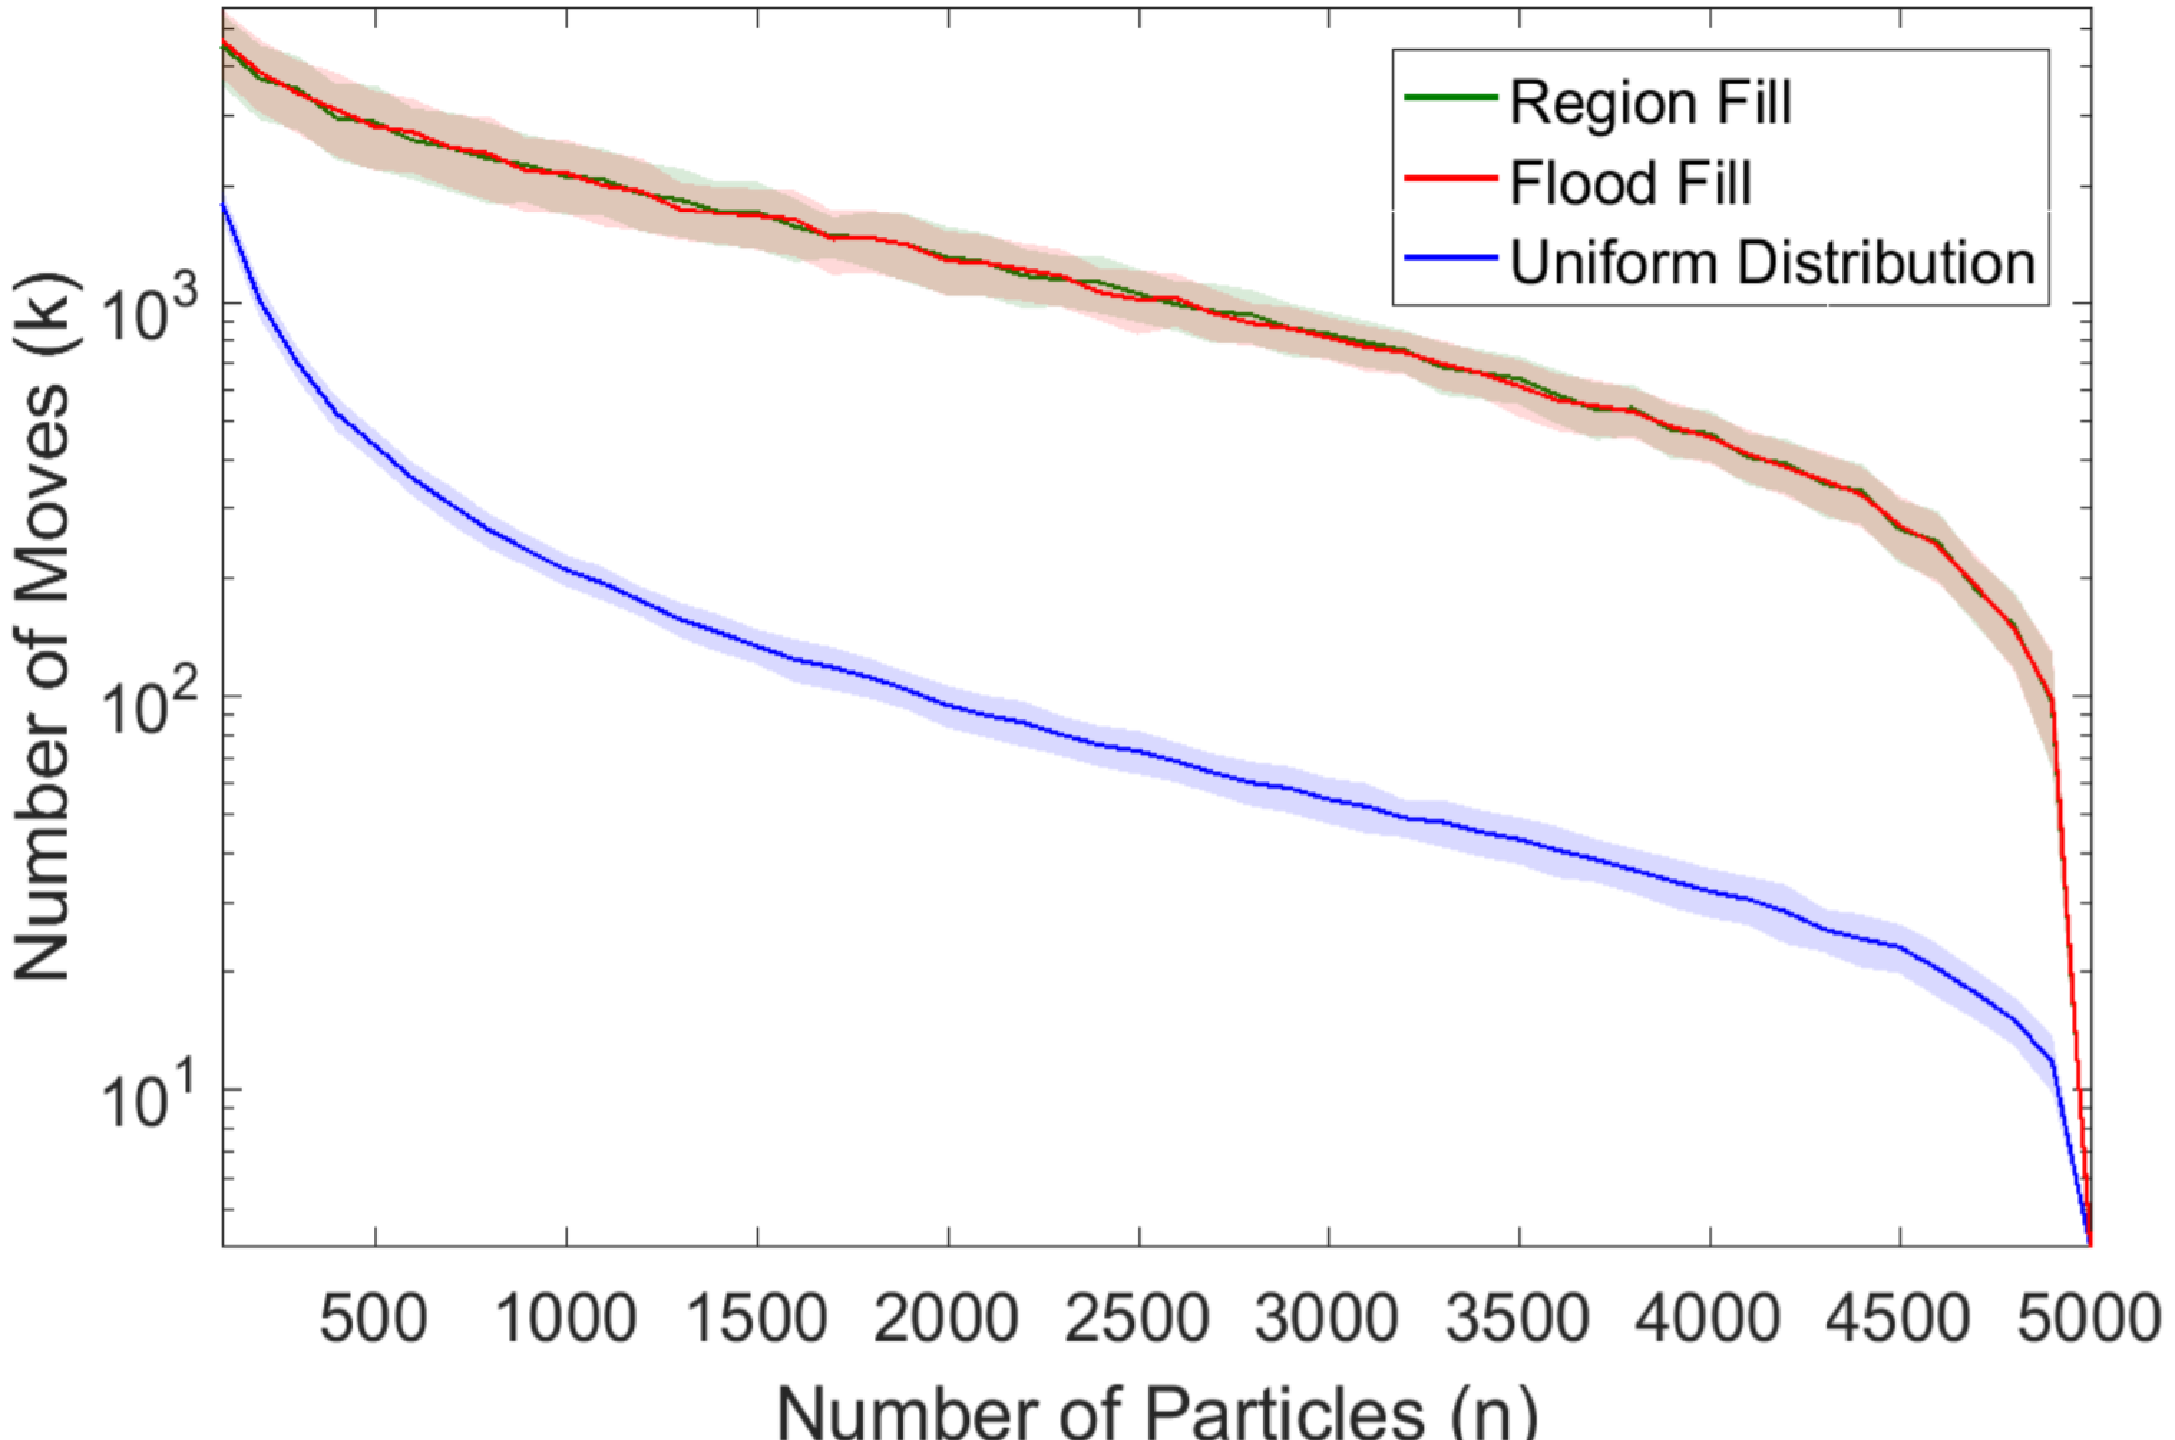
\includegraphics[width=1.0\columnwidth]{RegionvsFloodvsUniform.pdf}
\end{center}
\caption{\label{fig:RegionvsFloodvsUniform}
Comparison with different distributions:  flood-fill, region fill, and uniform distribution for mapping on the complex 2D map.}
\end{figure}


\begin{figure}
\begin{center}
	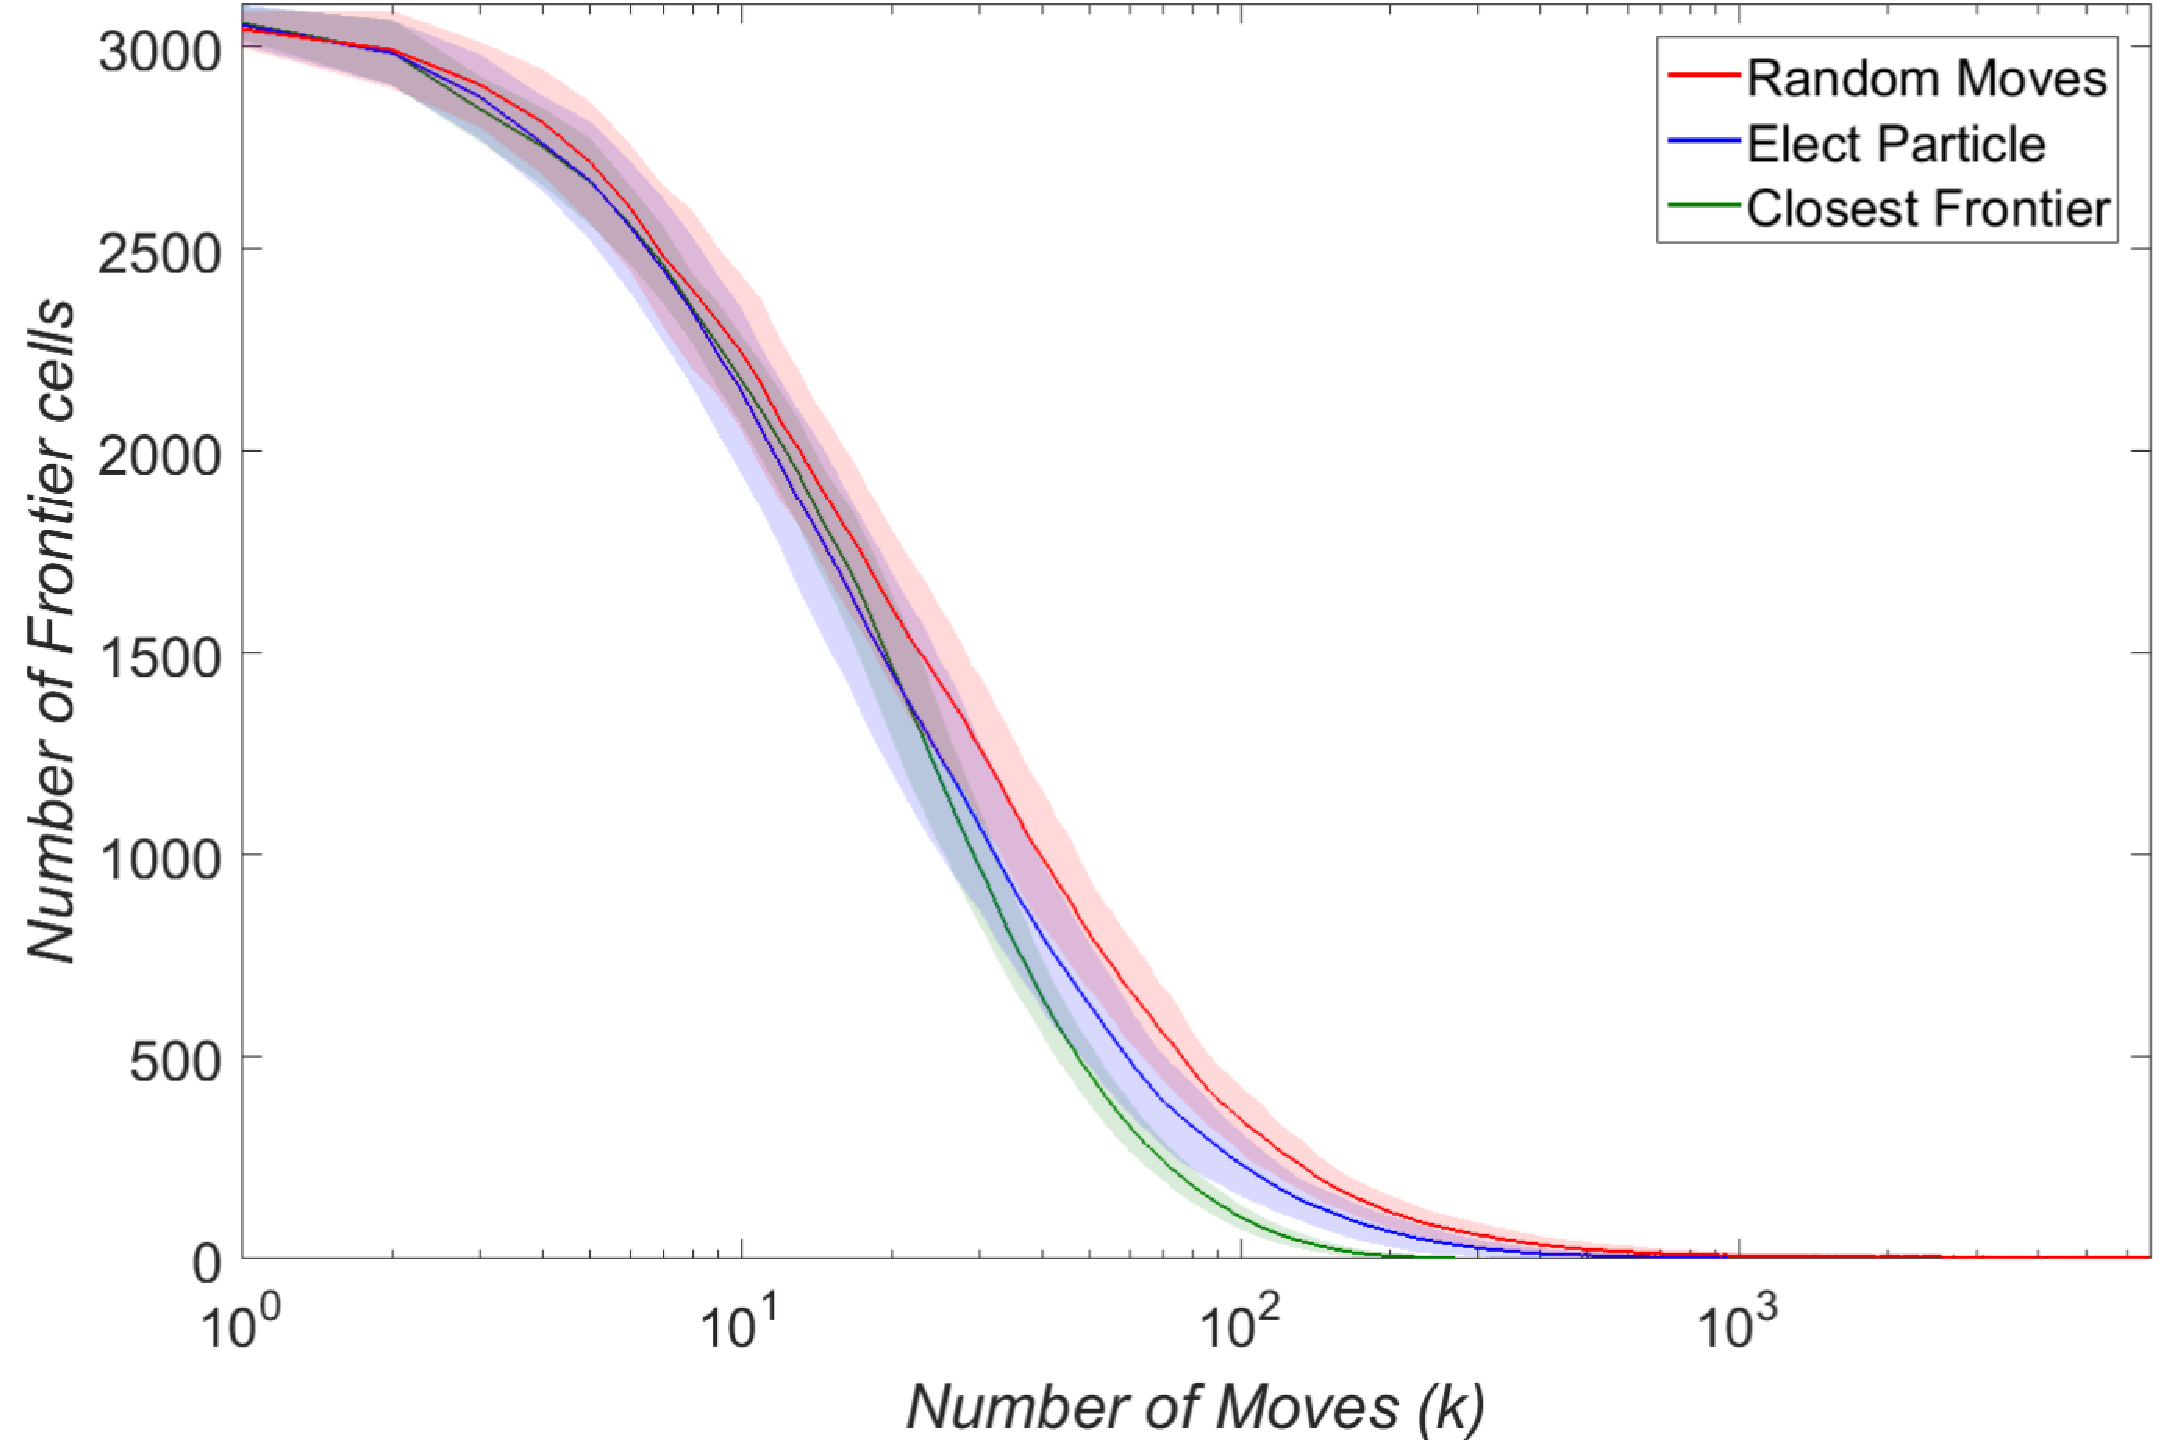
\includegraphics[width=1.0\columnwidth]{FrontierNodesVsk.pdf}
\end{center}
\caption{\label{fig:FrontierNodesVsk}
Performing mapping on the complex 2D map with $n=1000$ particles. Random moves requires an average of 4364 moves. Elect particle requires 933 moves and Closest Frontier requires 438 moves}
\end{figure}


